%---------------------------------------------------------------------------
\documentclass%%
%---------------------------------------------------------------------------
  [fontsize=11pt,%%          Schriftgroesse
%---------------------------------------------------------------------------
% Satzspiegel
   paper=a4,%%               Papierformat
   %enlargefirstpage=on,%%    Erste Seite anders
   %pagenumber=headright,%%   Seitenzahl oben mittig  
%---------------------------------------------------------------------------
% Layout
   headsepline=off,%%         Linie unter der Seitenzahl
   parskip=half,%%           Abstand zwischen Absaetzen
%---------------------------------------------------------------------------
% Was kommt in den Briefkopf und in die Anschrift
   fromalign=right,%%        Plazierung des Briefkopfs
   fromphone=off,%%           Telefonnummer im Absender
   fromrule=off,%%     Linie im Absender (aftername, afteraddress)
   fromfax=off,%%            Faxnummer
   fromemail=off,%%           Emailadresse
   fromurl=off,%%            Homepage
   fromlogo=on,%%            Firmenlogo
   addrfield=on,%%           Adressfeld fuer Fensterkuverts
   backaddress=on,%%         ...und Absender im Fenster
   subject=beforeopening,%%  Plazierung der Betreffzeile
   locfield=narrow,%%        zusaetzliches Feld fuer Absender
   foldmarks=on,%%           Faltmarken setzen
   numericaldate=off,%%      Datum numerisch ausgeben
   refline=narrow,%%         Geschaeftszeile im Satzspiegel
   firstfoot=on,%%           Footerbereich
%---------------------------------------------------------------------------
% Formatierung
   draft=off%%                Entwurfsmodus
]{scrlttr2}

%---------------------------------------------------------------------------
\usepackage[english, ngerman]{babel}  
\usepackage{url}
\usepackage{graphicx}
\usepackage[utf8]{inputenc} 
\usepackage[T1]{fontenc}
\usepackage[semibold]{raleway} 
\usepackage[ngerman]{babel}
\defaultfontfeatures{Ligatures={TeX}}
\renewcommand{\familydefault}{\sfdefault}
% symbols: (cell)phone, email
\RequirePackage{marvosym} 
% for gray color in header
\RequirePackage{color}

%---------------------------------------------------------------------------
% Meine zusätzlichen Befehle und Pakete
\usepackage{ragged2e}
\RaggedRightRightskip=0pt plus 4em % Flatterzone etwas größer als normal
\usepackage{pdfpages}
%---------------------------------------------------------------------------

%---------------------------------------------------------------------------
% Schriften werden hier definiert
\renewcommand*\familydefault{\sfdefault} % Latin Modern Sans
\setkomafont{fromname}{\sffamily}
%\setkomafont{pagenumber}{\sffamily}
\setkomafont{subject}{\mdseries}
\setkomafont{backaddress}{\mdseries}
\setkomafont{fromaddress}{\small\sffamily\mdseries}
%---------------------------------------------------------------------------
\begin{document}
%---------------------------------------------------------------------------
% Briefstil und Position des Briefkopfs
\LoadLetterOption{DIN} %% oder: DINmtext, SN, SNleft, KOMAold.
\makeatletter
\@setplength{sigbeforevskip}{17mm} % Abstand der Signatur von dem closing
\@setplength{firstheadvpos}{17mm} % Abstand des Absenderfeldes vom Top
\@setplength{firstfootvpos}{375mm} % Abstand des Footers von oben
\@setplength{firstheadwidth}{\paperwidth}
\@setplength{locwidth}{70mm}   % Breite des Locationfeldes
\@setplength{locvpos}{65mm}    % Abstand des Locationfeldes von oben
\ifdim \useplength{toaddrhpos}>\z@
  \@addtoplength[-2]{firstheadwidth}{\useplength{toaddrhpos}}
\else
  \@addtoplength[2]{firstheadwidth}{\useplength{toaddrhpos}}
\fi
\@setplength{foldmarkhpos}{6.5mm}
\makeatother
%---------------------------------------------------------------------------
% Farben werden hier definiert
% define gray for header
\definecolor{mygray}{gray}{.55}
% define blue for address
\definecolor{myblue}{rgb}{0.25,0.45,0.75}

%---------------------------------------------------------------------------
% Absender Daten
\setkomavar{fromname}{Björn Kawecki}
\setkomavar{fromaddress}{Große-Leege-Straße 14\\13055 Berlin}
%\setkomavar{fromphone}[]{+49\,(0)\,157\,52\,53\,30\,12}
%\setkomavar{fromfax}[\FAX~]{+49\,(0)\,123\,456\,789\,1}
%\setkomavar{fromemail}[]{bjoern.kawecki@mailbox.org}
%\setkomavar{fromurl}[]{http://ichunddu.de}
%\setkomafont{fromaddress}{\small\rmfamily\mdseries\slshape\color{myblue}}

\setkomavar{backaddressseparator}{ - }
%\setkomavar{backaddress}{Tim Metzner, Felderhof 112, 40880 Ratingen} % wenn erwünscht kann hier eine andere Backaddress eingetragen werden
%\setkomavar{signature}{Björn Kawecki}
\setkomavar{signature}{%
  
\includegraphics[height=25pt, angle=-3]{sig.png}\\
  Björn Kawecki}
\makeatletter% entfällt in der lco-Datei
\@setplength{sigbeforevskip}{16pt}
\makeatother% entfällt in der lco-Datei
% signature same indention level as rest
\renewcommand*{\raggedsignature}{\raggedright}
\setkomavar{location}{\raggedleft

%Kundennummer: 12345678 \\
%Ihr Zeichen:  asd123 \\
}

% Anlage neu definieren
\renewcommand{\enclname}{Anlagen}
\setkomavar{enclseparator}{: }
%---------------------------------------------------------------------------
% Seitenstil
%pagenumber=footmiddle
\pagestyle{plain}%% keine Header in der Kopfzeile bzw. plain
\pagenumbering{arabic}
%---------------------------------------------------------------------------
%---------------------------------------------------------------------------
%\firstfoot{\footnotesize%
%\rule[3pt]{\textwidth}{.4pt} \\
%\begin{tabular}[t]{l@{}}% 
%\usekomavar{fromname}\\
%\usekomavar{fromaddress}\\
%\end{tabular}%
%\hfill
%\begin{tabular}[t]{l@{}}%
%  \usekomavar[\Mobilefone~]{fromphone}\\
%   \usekomavar[\Letter~]{fromemail}\\
%\end{tabular}%
%\ifkomavarempty{frombank}{}{%
%\hfill
%\begin{tabular}[t]{l@{}}%
%\usekomavar{frombank}
%\end{tabular}%
%}%
%}% 
%---------------------------------------------------------------------------
% Bankverbindung
%\setkomavar{frombank}{Kto. 123456789\\
%BLZ 123\,123\,12\\
%Musterbank}
%---------------------------------------------------------------------------
%\setkomavar{yourref}{}
%\setkomavar{yourmail}{}
%\setkomavar{myref}{}
%\setkomavar{customer}{}
%\setkomavar{invoice}{}
%---------------------------------------------------------------------------
% Datum und Ort werden hier eingetragen
\setkomavar{date}{\today}
\setkomavar{place}{Berlin}
%---------------------------------------------------------------------------

%---------------------------------------------------------------------------
% Hier beginnt der Brief, mit der Anschrift des Empfängers

\begin{letter}
{
Werkbank GmbH\\
Viktoriastr. 75\\
44787 Bochum\\
}
%---------------------------------------------------------------------------
% Der \begin{center}
%•
%\end{center}Betreff des Briefes
\setkomavar{subject}{\textbf{Bewerbung: Django- / Python-Entwickler}}
%---------------------------------------------------------------------------
\opening{Sehr geehrtes Recruiting-Team,}
\RaggedRight% Rausatz statt Flattersatz.

ich bin autodidaktischer Programmierer mit geisteswissenschaftlichem Hintergrund und strebe den Einstieg in die professionelle Webentwicklung an.

Ich verfüge über fundierte Erfahrung in den Programmiersprachen Python und JavaScript sowie in grundlegenden Webtechnologien wie HTML, CSS und Docker. Dazu beherrsche ich die Grundlagen von React, Vue, FastAPI und SQL.

Für mein Portfolio (siehe Exposé) habe ich eine innovative Lernplattform für mein ursprüngliches Spezialgebiet (russische Sprache) entwickelt und hierfür den Technologie-Stack Django, PostgreSQL, HTMX und Docker verwendet.

Über eine Gelegenheit, Sie in einem persönlichen Gespräch von meinen Kompetenzen zu überzeugen, freue ich mich sehr.

\closing{Mit freundlichen Grüßen}
%---------------------------------------------------------------------------
%\ps{PS:}
\encl{Lebenslauf, Projekt-Exposé}
%\cc{}
%---------------------------------------------------------------------------
\end{letter}%---------------------------------------------------------------------------
%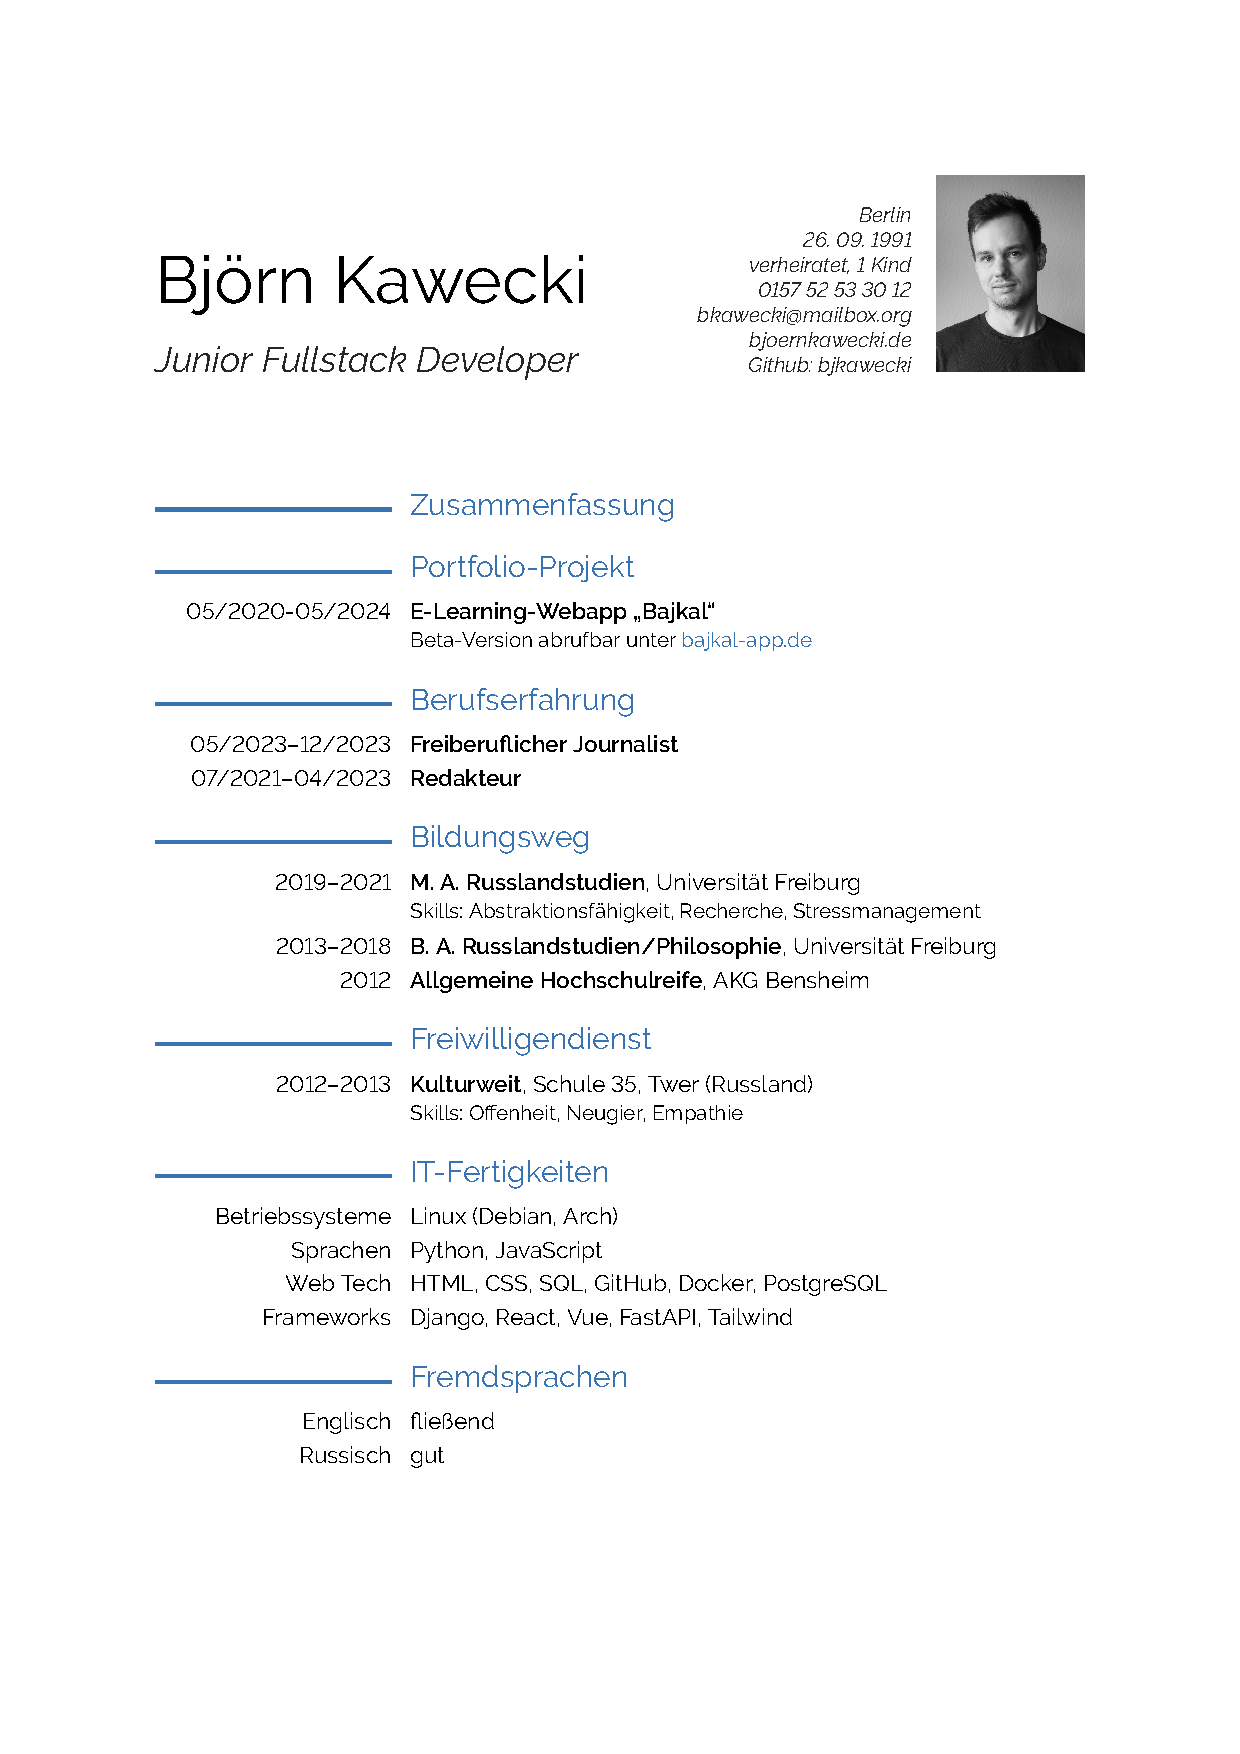
\includepdf[pages=-]{cv.pdf}
%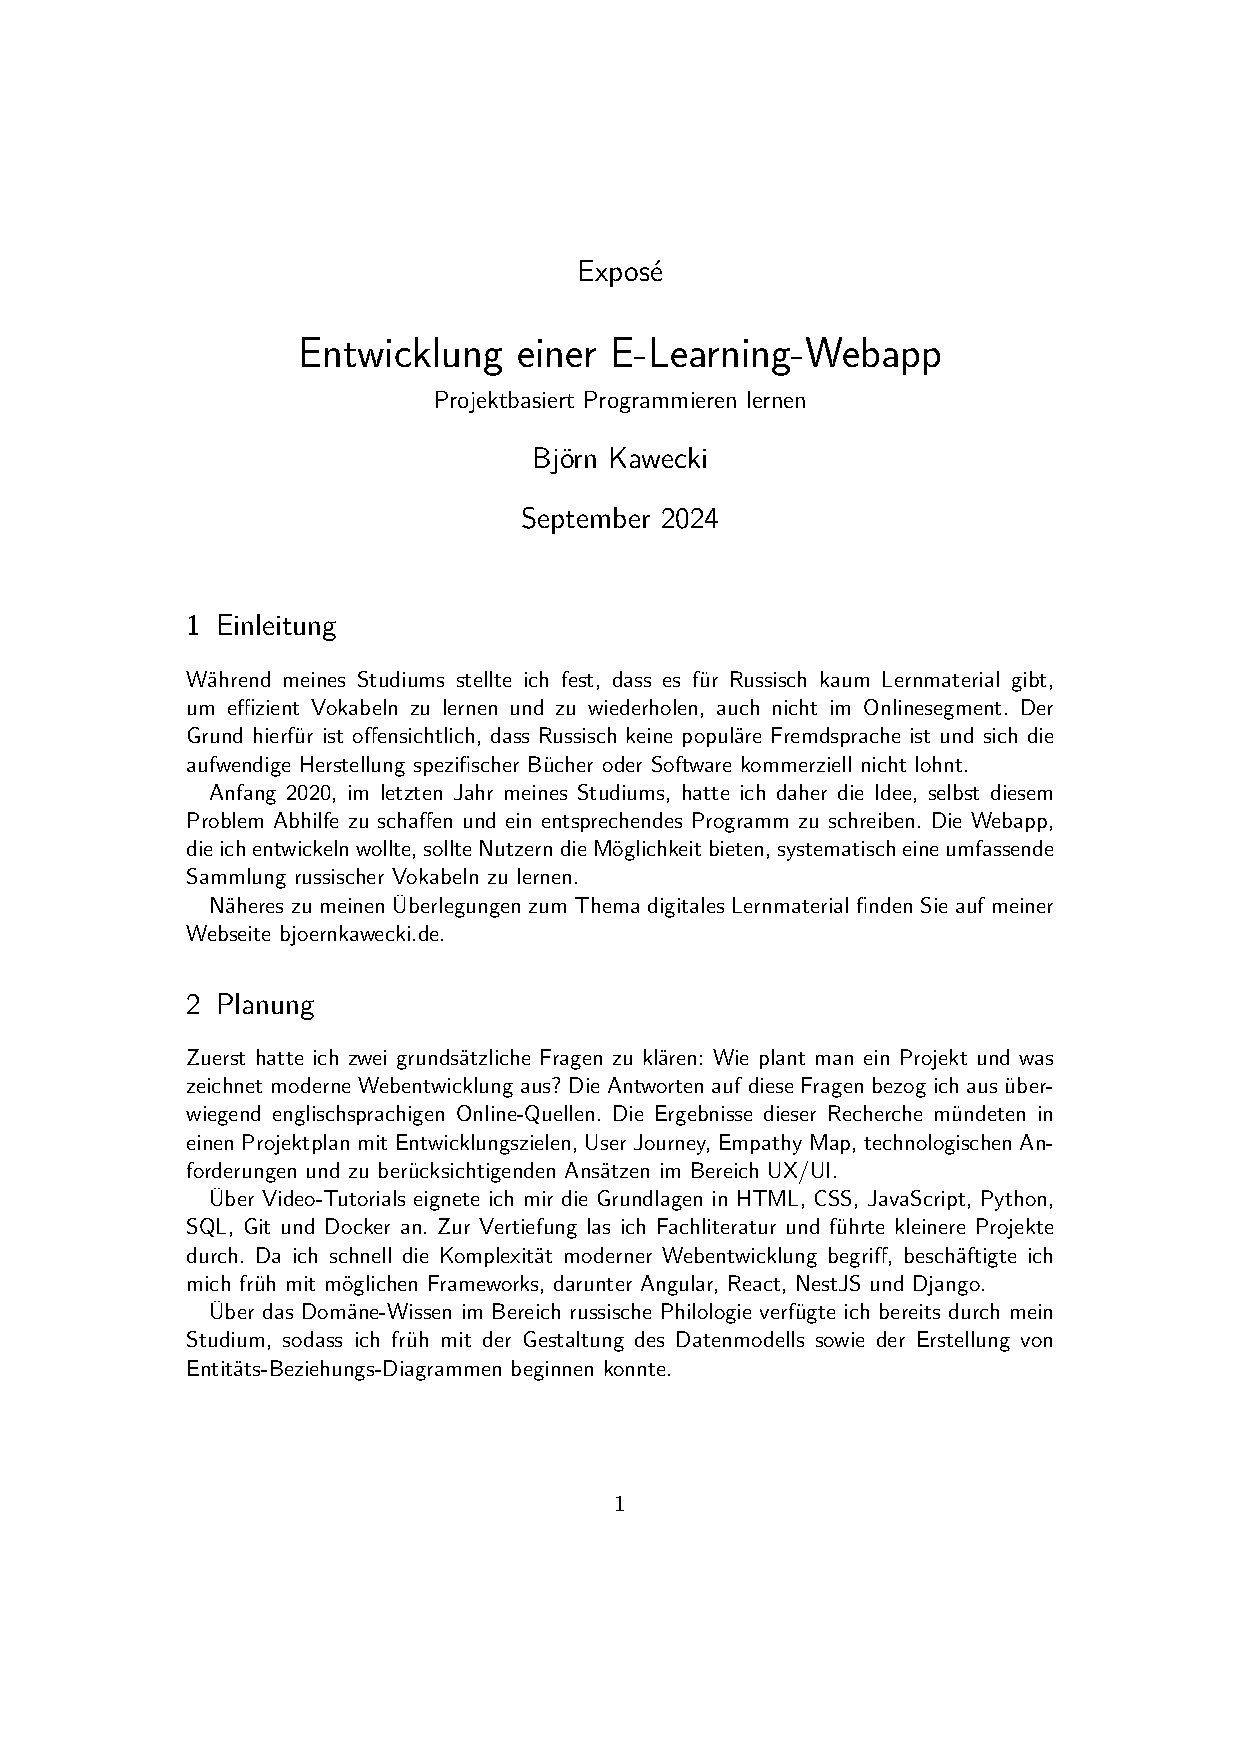
\includepdf[pages=-]{expose.pdf}

\end{document}
%---------------------------------------------------------------------------